\newchapt{Introduction}{chapt1}{Introduction}

The 3D modeling of urban buildings is an area of active research
with increasing attention drawn from the computer graphics and
computer vision communities.
Current state-of-the-art algorithms include procedural modeling,
3D laser scanning, and image-based approaches.
In addition, conventional modeling tools are commonly used for this purpose.
The most accurate input source for modeling {\it existing} buildings, though,
remains laser range scanners.
They provide high geometric detail by collecting range data from hundreds
of meters away with an accuracy on the order of a few millimeters.
This fidelity is appropriate for construction, architecture, cultural
heritage, and forensics applications.
Unfortunately, laser range scanning can produce an overwhelming amount of data,
which poses great challenges to visualization software that require lightweight
3D models for interactive use.
Polygonal data generated from range scans are therefore too dense for use in
web-based applications such as Google Earth and Microsoft Virtual Earth.
These applications work best with lightweight models consisting of only
hundreds of polygons.

The goal of this work is to automatically produce high-quality
lightweight models of urban buildings from large-scale 3D range data.
The proposed solution is inspired by the simple paradigm embedded in
procedural modeling as well as interactive tools such as Google SketchUp.
The core of these methods is that a simple set of extrusion and taper
operations applied to 2D contours can grow a wide array of complex 3D urban
models.
We propose a reverse engineering approach to infer key cross-sectional
planar contours along with a set of extrusion and taper operations to derive
lightweight models that conform to the 3D range data.

The proposed algorithm can generate models across a wide spectrum of
resolutions.
A particularly useful feature of the algorithm is that it outperforms
existing approximation techniques by preserving the sharpness of the raw
data, even at low resolution.
The contribution of this work is that it combines the benefits of
\emph{a priori} knowledge of urban buildings and fast 2D image
processing techniques to perform 3D modeling of urban buildings directly
from point cloud data.
This offers the benefit of a cost-effective geometry compression
approach for voluminous range data within the domain of urban structures.
It can be applied to boost web-based 3D applications, virtual city touring,
and online gaming.

\section{Related Work}

In an attempt to steer clear of tedious and expensive hand-made models,
procedural modeling of buildings in \cite{PMB_MWH,PMB_WWS,PMB_PM} has been proposed.
By using an effective description language, buildings and streets of a virtual
city can be generated automatically.
The strength of this approach is that the description language can generate
a huge number of buildings and streets quickly and beautifully.
This is particularly useful for gaming and other computer graphics applications.
However, since the parameters used to generate the buildings are randomly
generated, the city generated with these buildings and streets is a virtual one.
This approach is not useful for attempting to model an {\it existing} building.
In order to do so, one has to manually specify the parameters of the building,
which is very cumbersome.
Our goal is to automatically infer the contours and extrusion/taper parameters
of an existing building directly from dense range data.

Reconstruction of 3D models from range data has been addressed in
\cite{RE_Fisher,RE_CLF,RE_CD} with applications in numerous research areas,
including computer-aided design (CAD), computer vision, architectural modeling,
and medical image processing.
In \cite{DP_OWYC}, the authors proposed a 3D building reconstruction from a
2D floorplan image.
With the help of a 2D floorplan image, both the interior and exterior of a
building can be reconstructed accordingly.
A survey on methods for generating 3D building models from architectural
floor plans is given in \cite{YIN09}.
However, reliance on 2D floor plans makes this approach too limiting for
most applications, including our project.
In \cite{RE_TOGSH}, known manufacturing features were used to infer the
3D structure of mechanical parts.
Their method benefits from the domain knowledge that most of the mechanical
parts consist of predefined structures, such as holes, bosses, and grooves.
Our work is partially motivated by this idea since it also incorporates
{\it a priori} knowledge about the construction of urban buildings for further
inference.
However, their method is based on predefined simple geometry structures and
the assumption that the input 3D data has no holes.
This hinders their approach for those applications with incomplete data.

Medical image processing techniques are usually dealing with low SNR data.
There has been a lot of work on the medical 3D image reconstruction as in
\cite{MIR_FJS, MIR_BMMNB, MIR_KL, MIR_SKJ, MIR_SMHC, MIR_BVC}.
The basic ideas behind these approaches
are 3D reconstruction from sliced or histologic images using interpolation techniques.
The statistical inference are also intensively used to infer the low SNR images. For example,
In \cite{MIR_FJS}, Sigworth tried to deal with low SNR image data using maximum-likehood approach.
Because most of the statistical processes are computational intensity,
these approaches usually are heavy-duty approaches in order to obtain accurate, high resolution models.

Multimodal data fusion is another approach for large-scale urban
environment modeling.
In \cite{UM_Zakhor,UM_HYN}, both air and ground data are fused, including
laser scans, camera images, and aerial images.
The LIDAR scans are used to create the models and the camera images are used
for texture mapping.
Citing the cumbersome and expensive use of laser scanners, the researchers
in \cite{AKBARZADEH06} propose an approach that relies solely on passive
sensors (cameras) mounted on a moving vehicle.
Dense 3D point cloud measurements are derived using their multiview stereo
module based on multiple plane sweeping directions.
In an attempt to compress the voluminous data produced in the method of
\cite{AKBARZADEH06}, Xiao et al. \cite{UM_XFTQ} introduced an alternate
approach for modeling facades along a street using prior knowledge about
the buildings.
They achieve geometry compression and deliver a clean approximation of the
facades by applying a combination of plane fitting and window detection.
Their method, however, relies on limited assumptions about the planarity of
the buildings.
The method introduced in this paper, however, places no such limitations.
We can handle facades of any shape that exploit extrusion and taper operations.

The ball-pivoting algorithm (BPA) \cite{BPA_BMRS} is an efficient technique
for meshing 3D point clouds to produce polygonal models.
The generated meshes, however, constitute heavyweight models,
with the number of vertices nearly approaching the number of points in the
3D point cloud.
This limits its usefulness for web-based applications.
Although a BPA model can be simplified using approximation techniques such as
{\it qslim} \cite{BPA_GH}, the sharp detail of the original model is not
preserved.

In addition to the aforementioned research projects carried on in academia, 
some commercial products are developed in start-up companies. 
In \cite{IND_YC}, the buildings in Manhanttan are modeled to enhance
the virtual reality of social network. The buildings are accurately modeled via
aerial LIDAR data and were associated with address and related social information.
The most related commercial product is EdgeWise\textsuperscript{\texttrademark}, 
a new developed product by ClearEdge\textsuperscript{3D} \cite{IND_EW}.
In EdgeWise integrated development environment (IDE), the 3D point data 
(in pts or ptz format) can be loaded and visualized. And then, as an initial step,
ground extraction is applied to classify the point cloud data. 
Essentially, the point cloud in the same planar are marked. 
The next step is to infer the polygons from the scan data based on the classification. 
Once the polygons are inferred, the model is
exported to CAD format (dxf) and can be edited in Google SchetchUp. 
As a matter of fact, the CAD model it produced contains a lot of noisy and spikes. 
Basically, this commercial tool provides a good starting point for editing. 
It can only handle planar at this point in time and 
the resolution of the model it generated is not adjustable.


%%%%%%%%%%%%%%%%%%%%%%%%%%%%%%%%
%%%%%%   Overview  %%%%%%%%
%%%%%%%%%%%%%%%%%%%%%%%%%%%%%%%%
\section{Overview}

We propose an efficient way to reconstruct 3D models from range data by
partitioning the data into thin cross-sectional volumetric slabs.
For each slab, all range data in that slab is projected onto a 2D
cross-sectional contour slice.
Producing this array of slices permits us to avoid costly computation directly
on 3D data.
A similarity measure \cite{IR_Brown, IR_ZF, RE_WWLZ} is used to 
cluster the sliced images together into {\it keyslices}.
This term is analogous to the use of ``keyframes'' in computer animation,
which denotes important snapshots in the animation sequence from which
intermediate results can be derived.
In essence, each keyframe is a slice in the spatiotemporal volume of
an animation.
Similarly, each keyslice is a 2D image which contains a {\it transitional}
cross-section of the building, encapsulating major contours in the facade.
The model is then generated by applying basic extrusion and taper
operations from one keyslice to the next.
This produces a lightweight representation consisting of only a few
hundred polygons.

\begin{figure}[htb]
  \centering
  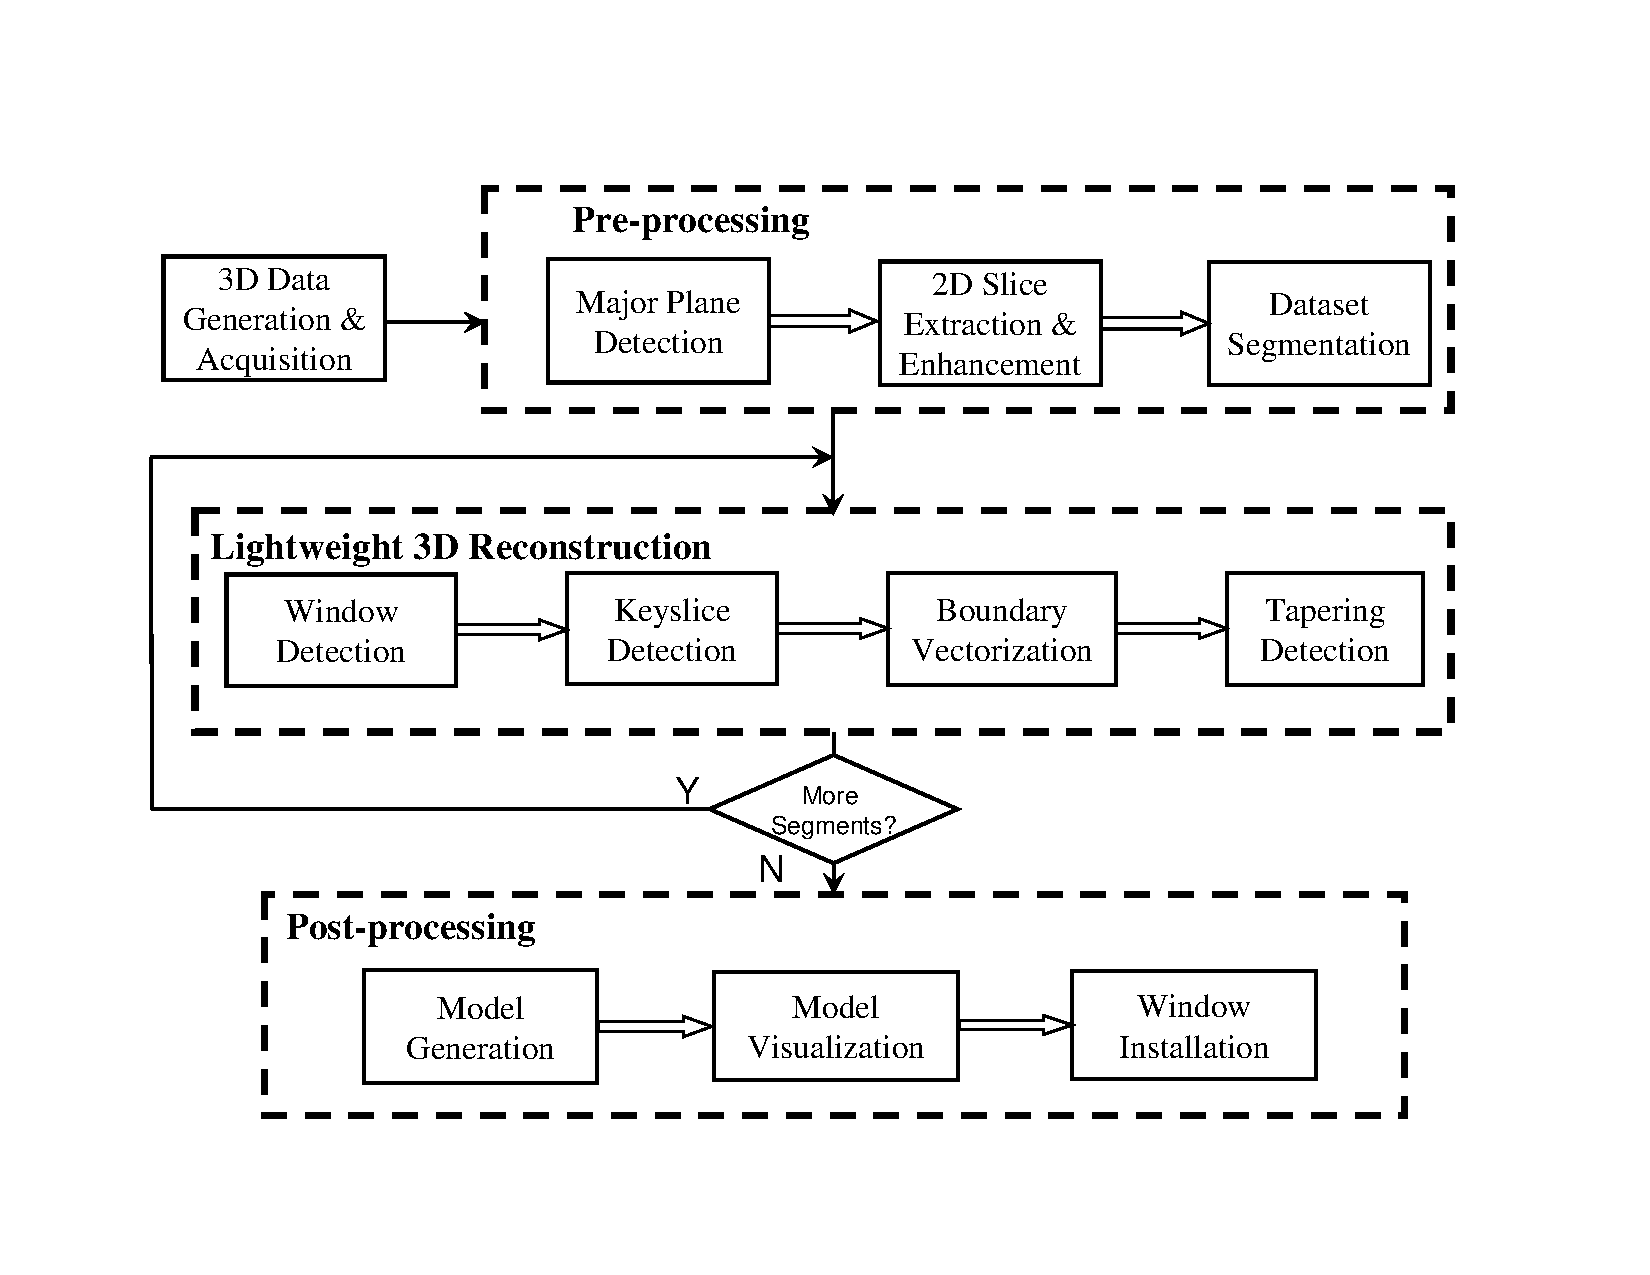
\includegraphics[width=\textwidth]{flow.pdf}
      \caption{Flow graph for proposed approach}
      \label{fig:flow}
\end{figure}

An overview of our approach, depicted in \Fig{ov}, begins with the
acquisition of a dense 3D point cloud $C$ of a building.
$C$ is then partitioned into a nonoverlapping set of volumetric slabs.
Each slab $S$ is associated with one projection plane $P$,
sitting at the base of $S$.
The purpose of partitioning $C$ is to establish a set of cross-sections,
or contour slices.
By examining the changes among these slices, we can identify the prominent
slices, or {\it keyslices}, as well as the necessary extrusion and
taper operations that must apply to them to generate the model.
By casting this 3D modeling task into a series of 2D operations, we
reduce the dimension of the problem to achieve a significant savings in
computational complexity.

To generate the 3D model of a building, all these key raster images need 
to be vectorized to represent the silhouette or boundary of the building. 
Couple of raster image vectorization approaches are
proposed in \cite{DP_AAKMT, DP_DP, DP_WM}. The Douglas-Peucker
algorithm tried to connect all the existed points to form a polygon. 
Although the implementation of
this approach is very efficient with the improvement in \cite{DP_HS},  this method cannot
handle the case where some extra interior points are existed as some outlier data.
To tackle this issue, Medeiros et al. \cite{BPA_MVL} applied ball-pivot algorithm (BPA)
\cite{BPA_BMRS}, which was original proposed on 3D point cloud data, on the 2D image to obtain
vectorized boundary. The key parameter for BPA to work successfully is to find the right size of
the ball for pivoting. We have proposed an adaptive BPA algorithm to solve this problem.

\begin{figure}[htbp]
\begin{center}
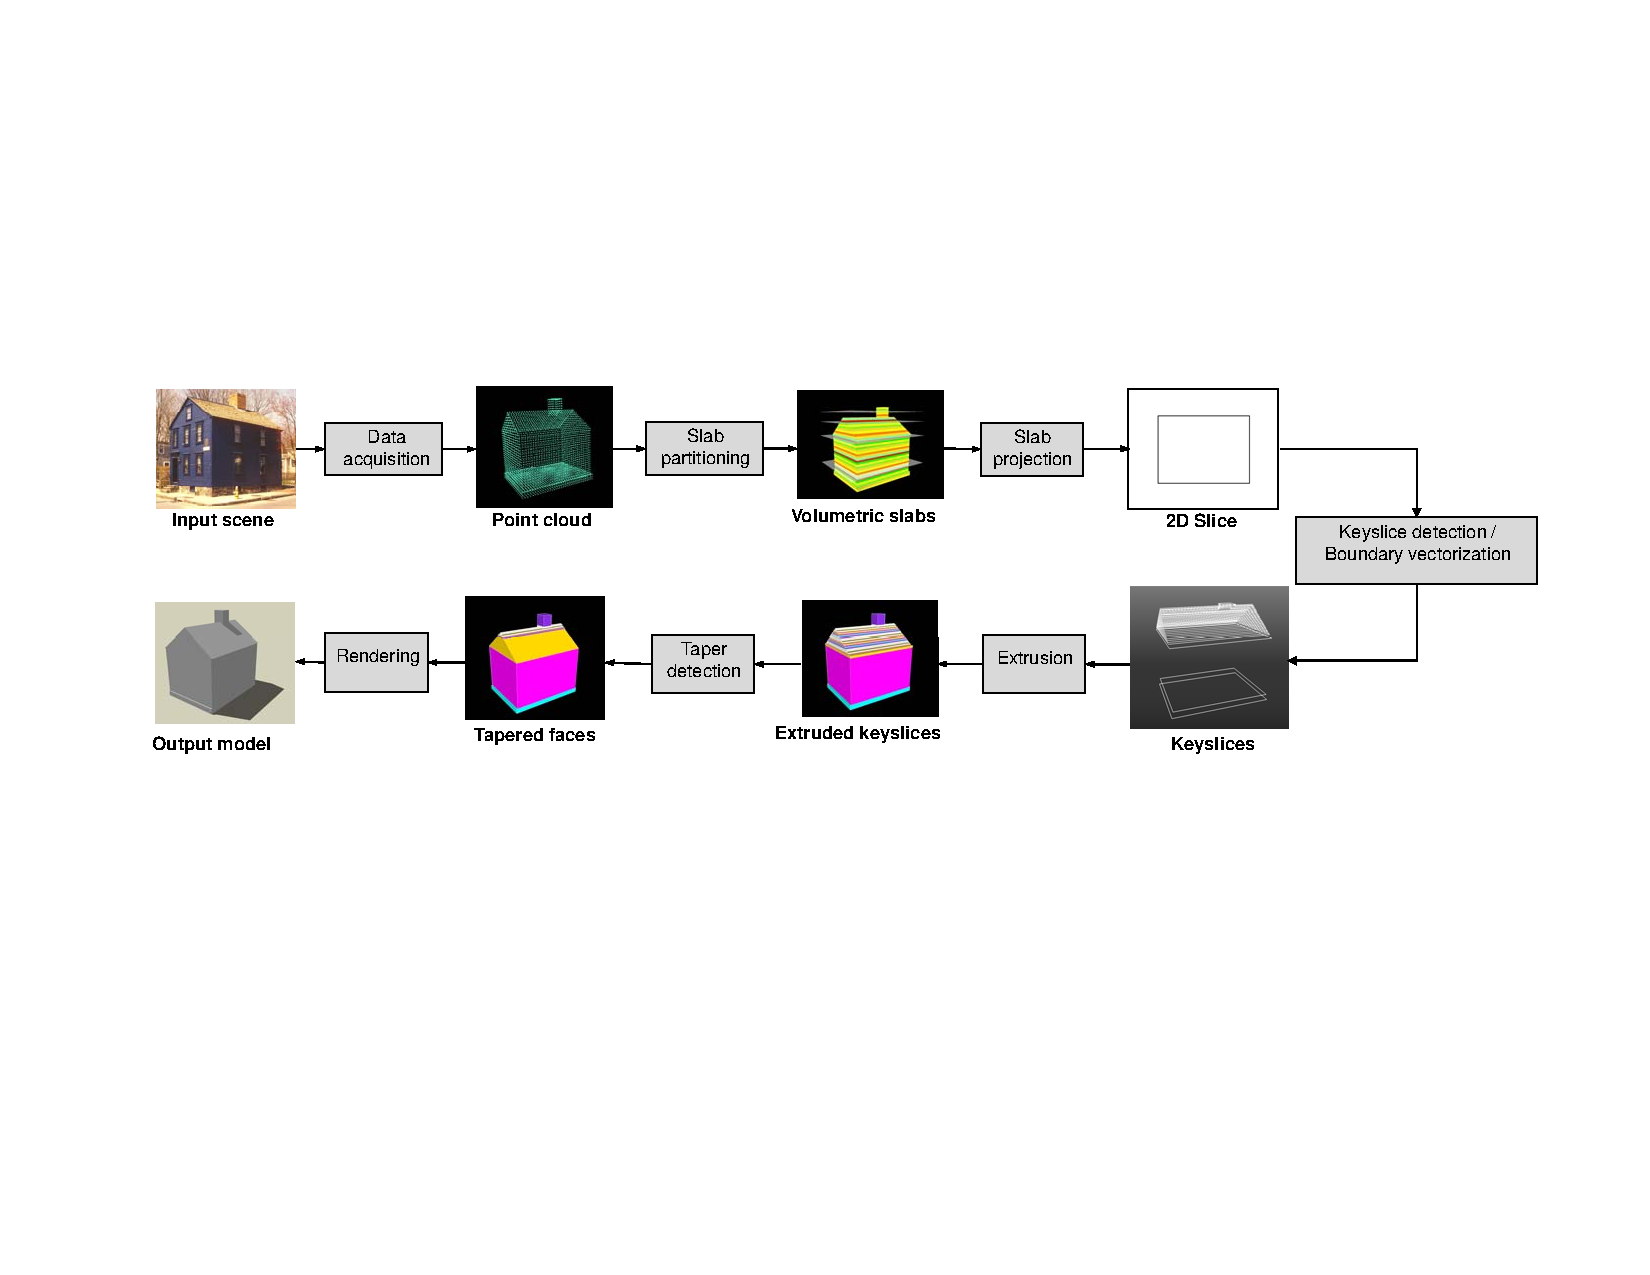
\includegraphics[width=1.0\textwidth]{overview.pdf}
\end{center}
\caption{Overview of the proposed approach.}
\label{fig:ov}
\end{figure}

Due to occlusion and material-dependent reflection problems off of glass
(e.g., windows), the input data is incomplete and noisy.
Therefore, noise removal and hole filling are carried out as a
preprocessing stage to generate the 3D model.
The next stage of the approach is to carry out fast image processing
techniques on the enhanced image slices to detect keyslices.
Boundary vectorization for these raster keyslices is then conducted to
transform these points into polygons.
Tapered structure detection is carried out to further reduce the model size.
Finally, 3D model generation is achieved by applying the extrusion/taper
operations to the keyslices to reconstruct lightweight 3D models of urban
buildings from range data.

\newchapt{Preprocessing on Range Data}{chapt2}{Preprocessing on Range Data}

%%%%%%%%%%%%%%%%%%%%%%%%%%%%%%%%
%%%%%%   PREPROCESSING  %%%%%%%%
%%%%%%%%%%%%%%%%%%%%%%%%%%%%%%%%
%\section{Preprocessing the Range Data}
\label{sec:prep}

The input to our system is range data assembled as a 3D point cloud.
Our data is obtained from a Leica Cyrax 2500 laser range scanner \cite{RDP_LRS},
which works by sweeping an eye-safe laser beam across the scene to collect
up to one million 3D depth points per frame.
All scene points that lie within 100 meters can be acquired with an accuracy
of 5mm in depth.
The basic algorithm that we use for registering the voluminous 3D data
acquired from multiple scans of buildings has been introduced in
\cite{RDP_LS}.
That same algorithm is also responsible for extracting the major axes
of the building in order to align it to the axes of the world coordinate
system.
This is necessary to properly infer the keyslices.
\Figb{IR_2_DXF} displays a properly aligned, {\it registered} 3D point cloud
consisting of 14 scans totalling 14 million points.

\begin{figure}[htbp]
\begin{center}
\begin{tabular}{c}
	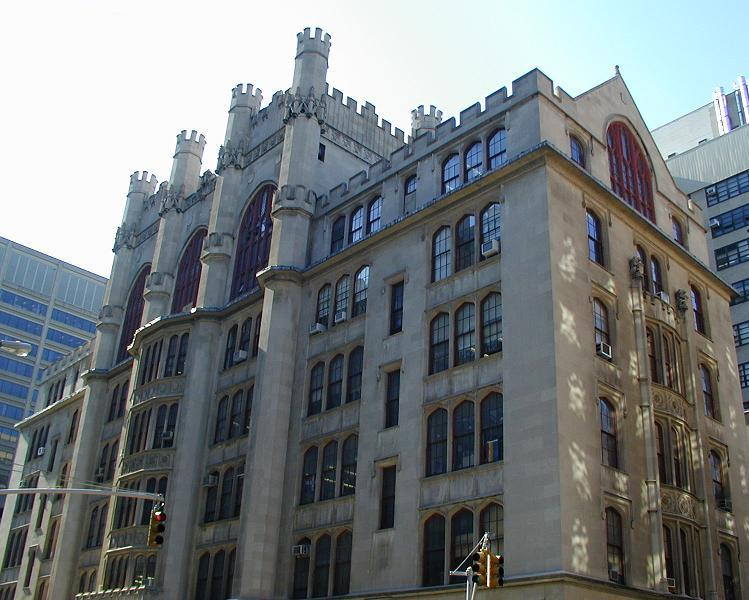
\includegraphics[width=0.6\textwidth]{HunterPhoto.jpg} \\
	(a)\\
	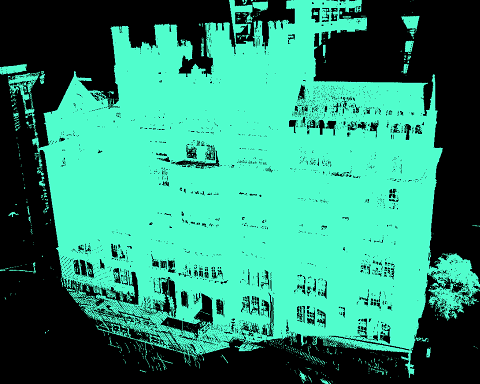
\includegraphics[width=0.6\textwidth]{point_cloud.png} \\
	(b)
\end{tabular}
\end{center}
\caption{
(a) Image of building to be modeled.
(b) 3D point cloud of building assembled by registering multiple scans.
}
\label{fig:IR_2_DXF}
\end{figure}

Due to occlusions and limited vantage points, the point cloud collected by the
laser scanner contains artifacts and holes.
In addition, computing directly on 3D data is time-consuming and
computationally complex.
To tackle these issues, we define inner and outer bounding boxes for the
building to clip away unrelated scene objects.
Then, we convert the 3D modeling problem into a set of 2D problems by
projecting the 3D data into a series of 2D cross-sectional contour images.
Noise removal, hole filling, and vectorization are all done in this
2D space.

%%%%%%%%%%%%%%%%%%%%%%%%%%%%%%%%
%%%%%% 3D Data Rectification %%%
%%%%%%%%%%%%%%%%%%%%%%%%%%%%%%%%
\section{Point Cloud Rectification}
\label{sec:rect}

%% Put the flow of the data rectification.
Although the multiple scans of point cloud data have been registered, 
they are not rectified as depicted in \Fig{pc_orig}. 
Please note the point cloud has been sub-sampling by a factor of 50.
This is not suitable for our further 3D modeling.
As one of the pre-processing steps, this registered data will be rotated
and translated to be aligned with world coordinates.

%% Put the image of rectfied data.
\begin{figure}[htbp]
\begin{center}
\begin{tabular}{c}
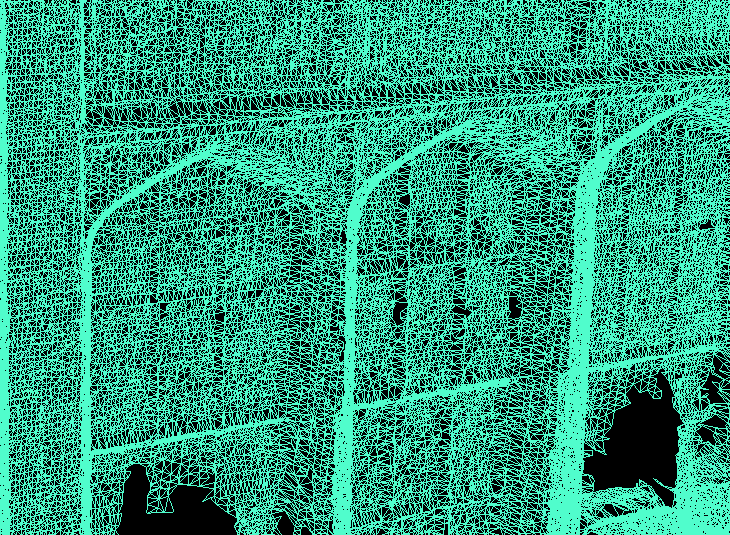
\includegraphics[width=\textwidth]{BPA_TH.png}
\end{tabular}
\end{center}
\caption{ The registered point cloud without rectification. }
\label{fig:pc_orig}
\end{figure}

As we know, there are a lot of line features existed in the point cloud, which
provides a good clue for rectifing the data. 
For each scan $s$ of the scene, we can obtain a set of line segments $L_s$. 
Assume $T_s$ is the transformation matrix for the scan $s$ to be registered with other scans.
In other words, for any point $P(x,y,z)$ in the scan $s$, $P*T_s$ will transform the
point $P$ into the final registered coordinate system as shown in \Fig{pc_orig}.

We can obtain the major axises by clustering these line segemetns $L_s$ from different
scans. The purpose of clustering is to group the lines whose direction are very close to each other.
To cluster these lines, we first transform the line segments in $L_s$ into world
corrdinate system using $T_s$ as described above. After transformation, we will
get a larger line set $L = {l_1, l_2, \ldots, l_n}$. For each line $l_i$, we first
normalize it to a unit vector:
\begin{equation*}
\bar{l_i} = \frac{l_i}{\parallel l_i \parallel}
\end{equation*}

The unit vector $\bar{l_i}$ has the unique length 1, which provides a good starting point 
for clustering since we do not need to worry the length of the lines. 
An array of bins are used to hold the unit vectors.
As the initial step, the first line $\bar{l}$ is picked up and is insert into the 
first bin and set the counter of the bin to 1.
When a new unit vector $\bar{l_n}$ is observed, we try to see whether there is an
existed unit vector in the bins which has similar direction as $\bar{l_n}$. This is
done by computing the distance $d_{\pm}=\parallel \pm\bar{l_n} - \bar{l_i} \parallel$.
Because $\bar{l_n}$ can has two opposite directions, we can compute both of them and
choose the smaller value as the distance $d$. If $d$ is smaller enough, $\bar{l_n}$
is clusterd with the line $\bar{l_i}$ and the counter of the bin holding $\bar{l_i}$
is increased by 1. On the other hand, if $d$ is big, we have to compare $\bar{l_n}$
with a line in the next bin. If $\bar{l_n}$ could not fit any line in the bins, we
will insert $\bar{l_n}$ into a new bin and set the counter of the bin to 1. 
To avoid the bias of the initial select, each unit vector $\bar{l_i}$ is
adjusted to be the mean of all unit vectors falling inside this bin. 

Once we go through all the lines in $L$, the clustering is complete. 
The next step is to choose the major axises from the clustering results. 
Essentially, this is to choose bins whose counters are among largest. 
Assume $u$, $v$, and $n$ represent the three largest bins. This is demonstrated in
\Fig{pc_orig} in red, green and blue respectively. To rectify the data,
we can refer to the following transformation matrix $\mathbf{M}$:
\begin{figure}[htbp]
\begin{center}
\begin{tabular}{c}
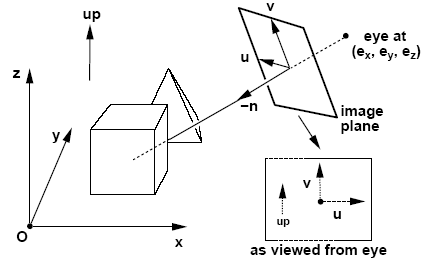
\includegraphics[width=0.5\textwidth]{point_cloud_rect_matrix.png}
\end{tabular}
\end{center}
\caption{ The transformation matrix. }
\label{fig:pc_rect_matrix}
\end{figure}

\begin{equation*}
\mathbf{M} = \left(
\begin{array}{cccc}
u_x & u_y & u_z & -e_x \\
v_x & v_y & v_z & -e_y \\
n_x & n_y & n_z & -e_z \\
  0 &   0 &   0 &    1 
\end{array} \right)
\end{equation*}

This is illustrated in \Fig{pc_rect_matrix}. $(x, y, z)$ is the world coordinate system.
The rectified coordinate system is represented using $(u, v, n)$. 
The vector $[-e_x, -e_y, -e_z]^T$ is the translation of the view point from the world origin.
After the transformation with $\mathbf{M}$, the new data set and the three major line segments are
shown in \Fig{pc_rect}.

%% rectified data
\begin{figure}[htbp]
\begin{center}
\begin{tabular}{c}
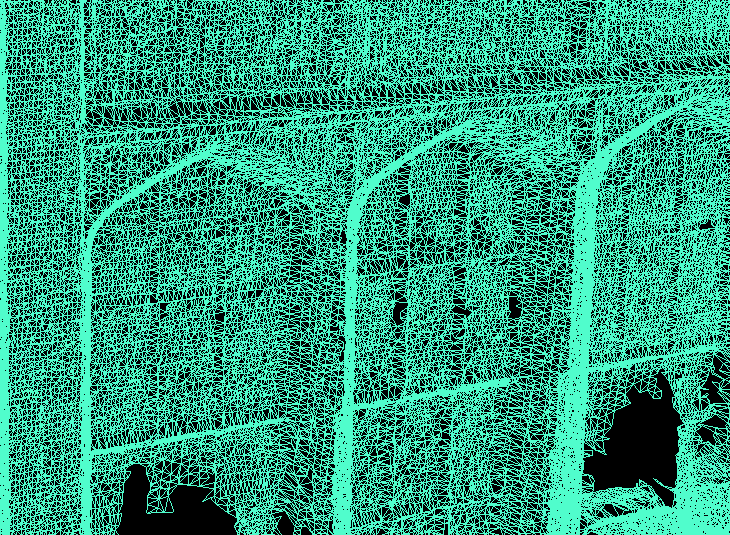
\includegraphics[width=\textwidth]{BPA_TH.png}
\end{tabular}
\end{center}
\caption{ The rectified point cloud of \Fig{pc_orig}. }
\label{fig:pc_rect}
\end{figure}


\section{Extraction of 2D Slices}
\label{sec:image_slicing}

We consider the point cloud data as a large array of 3D points to be
sliced into horizontal volumetric slabs.
All 3D points within each slab are projected onto a horizontal projection
plane, or slice, at the base of the slab.
\Fig{slice_slab} shows the 3D point cloud in \Figb{IR_2_DXF} partitioned into
50 slabs.
The 3D points in each slab are projected onto a projection plane to
form cross-sectional contour slices.
\Fig{slicing} depicts four such slices, associated with the four displayed
projection planes of \Fig{slice_slab}.

\begin{figure} [htbp]
\begin{center}
\begin{tabular}{c}
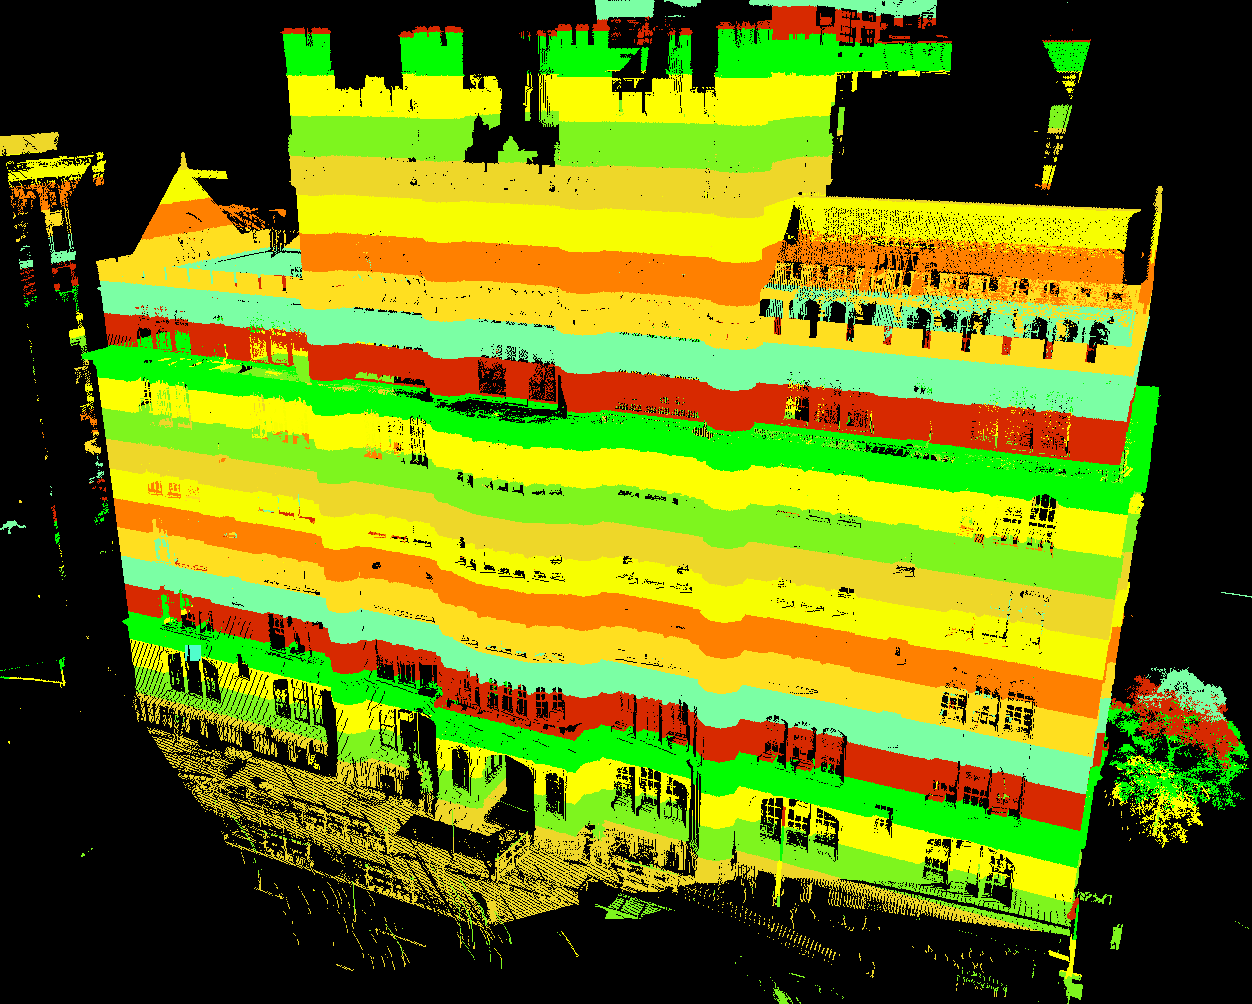
\includegraphics[width=0.6\textwidth]{slab_noplanar.png} \\
(a) \\
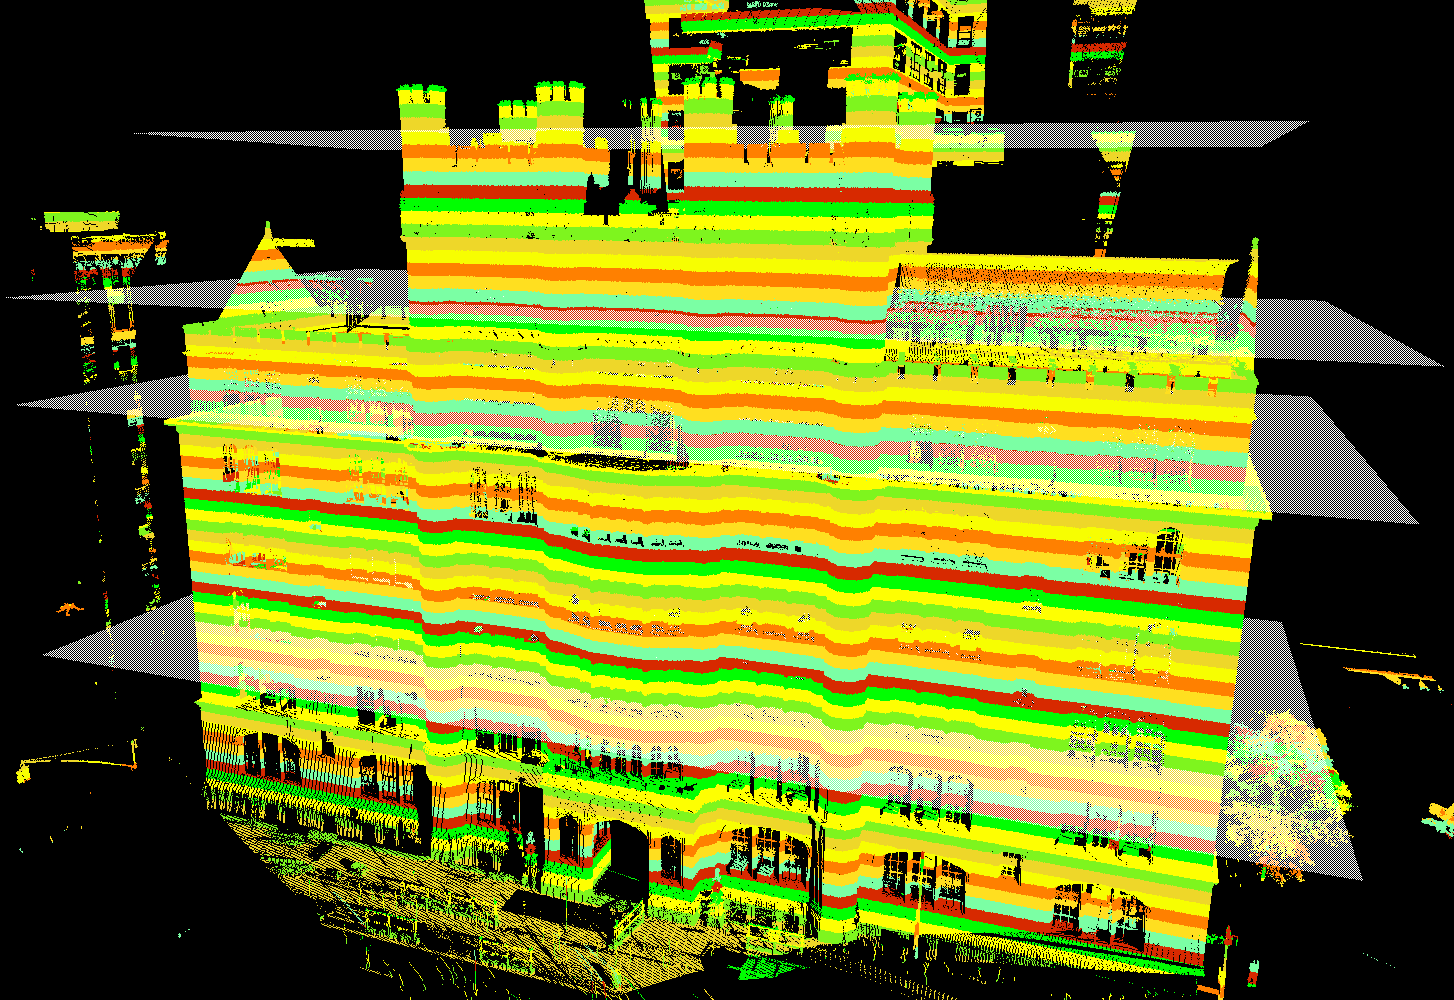
\includegraphics[width=0.6\textwidth]{slab_planar.png} \\
(b)
\end{tabular}
\end{center}
\caption{
(a) Slabs of the 3D point cloud data are used to determine prominent
cross-sections upon which extrusion/taper operations are applied.
(b)The 3D point cloud of \Figb{IR_2_DXF} partitioned into uniform
volumetric slabs.
The 3D points in each slab are projected onto a projection plane to
form cross-sectional slices. Four such planes are shown.}
\label{fig:slice_slab}
\end{figure}

The height of each slab is $\boldsymbol{\delta}$.
If $\boldsymbol{\delta}$ is held constant, each slice is generated from
equi-spaced slab intervals.
If $\boldsymbol{\delta}$ is allowed to vary, then we may
choose to allow for large values in parts of the structure that are similar,
and low values in regions that contain finer detail.
To avoid working on 3D data directly, a relatively small constant value
for $\boldsymbol{\delta}$ is chosen to generate 2D cross-sectional image slices.

\begin{figure} [htbp]
\begin{center}
\begin{tabular}{cc}
\fbox{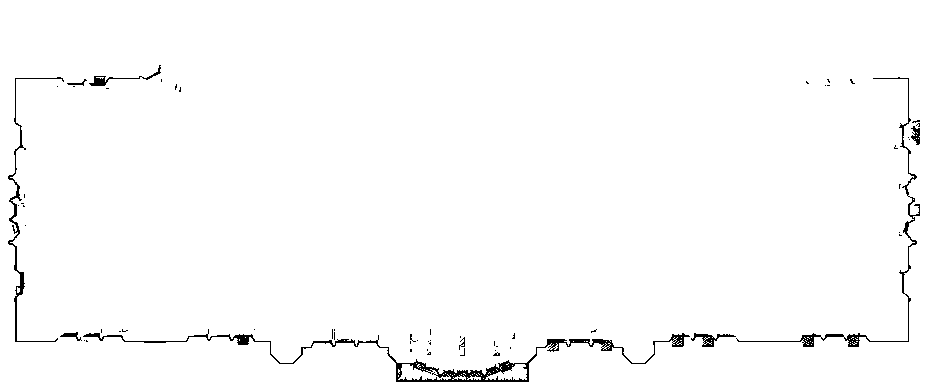
\includegraphics[width=0.45\textwidth]{image_slice_0190.png}} &
\fbox{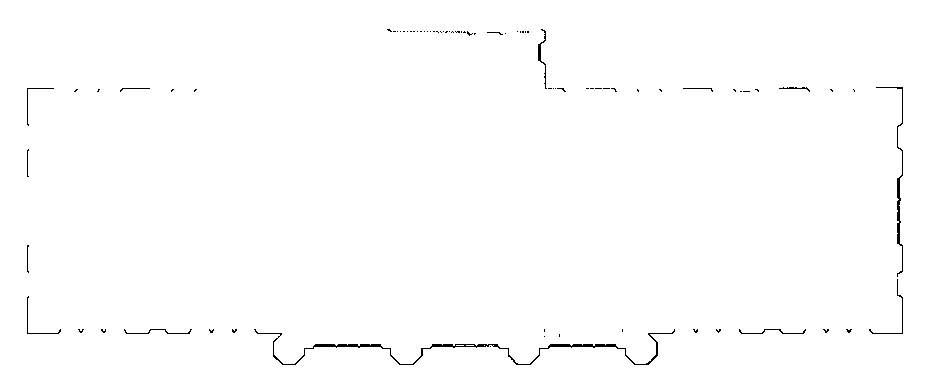
\includegraphics[width=0.45\textwidth]{image_slice_0600.png}} \\
(a) & (b) \\
\fbox{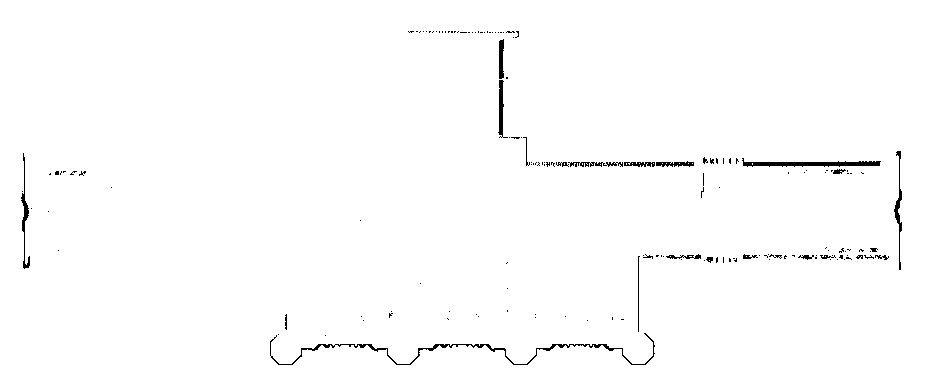
\includegraphics[width=0.45\textwidth]{image_slice_0714.png}} &
\fbox{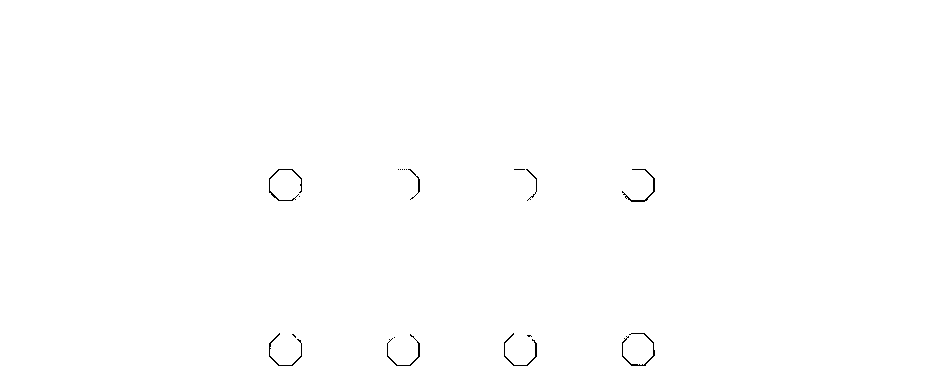
\includegraphics[width=0.45\textwidth]{image_slice_0951.png}} \\
(c) & (d)
\end{tabular}
\end{center}
\caption{The set of slices corresponding to the four projection planes in
\Fig{slice_slab}.}
\label{fig:slicing}
\end{figure}

Without loss of generality, the $y-$axis is used to represent the bottom-up
vertical direction.
Over each slab in height range $[H_{lo}, H_{hi})$,
we project the 3D data $\boldsymbol{P}(x,y,z)$, for $H_{lo} \leq y < H_{hi}$,
onto a 2D image slice.
The projection is normalized in the range $[0,W]$, where $W$ is the image width:
\begin{equation}
[\,x^{2D},\; y^{2D}\,]^T = \omega\cdot[\,x^{3D}_i - X_{MIN},\; z^{3D}_i - Z_{MIN}\,]^T
\label{eq:image_slicing}
\end{equation}
Note that $\omega = W/(X_{MAX} - X_{MIN})$, and that
the [$X_{MIN}$, $X_{MAX}$] and [$Z_{MIN}$, $Z_{MAX}$] pairs define the
3D bounding box, which can be obtained through user input and can be used
to clip away noise data.
\Fig{slicing}(a)-(d) show some examples of the 2D slices, where noise
and incomplete data are observed.

